\section{Experiments}
\label{sec:feats_results}
% We first give visual examples of our superpixel segmentation.

\subsection{Superpixel Segmentation}
\label{sec:superpix}
Fig. \ref{fig:sp_example} shows examples of the superpixel segmentation.

\begin{figure}[htbp]
  \centering
  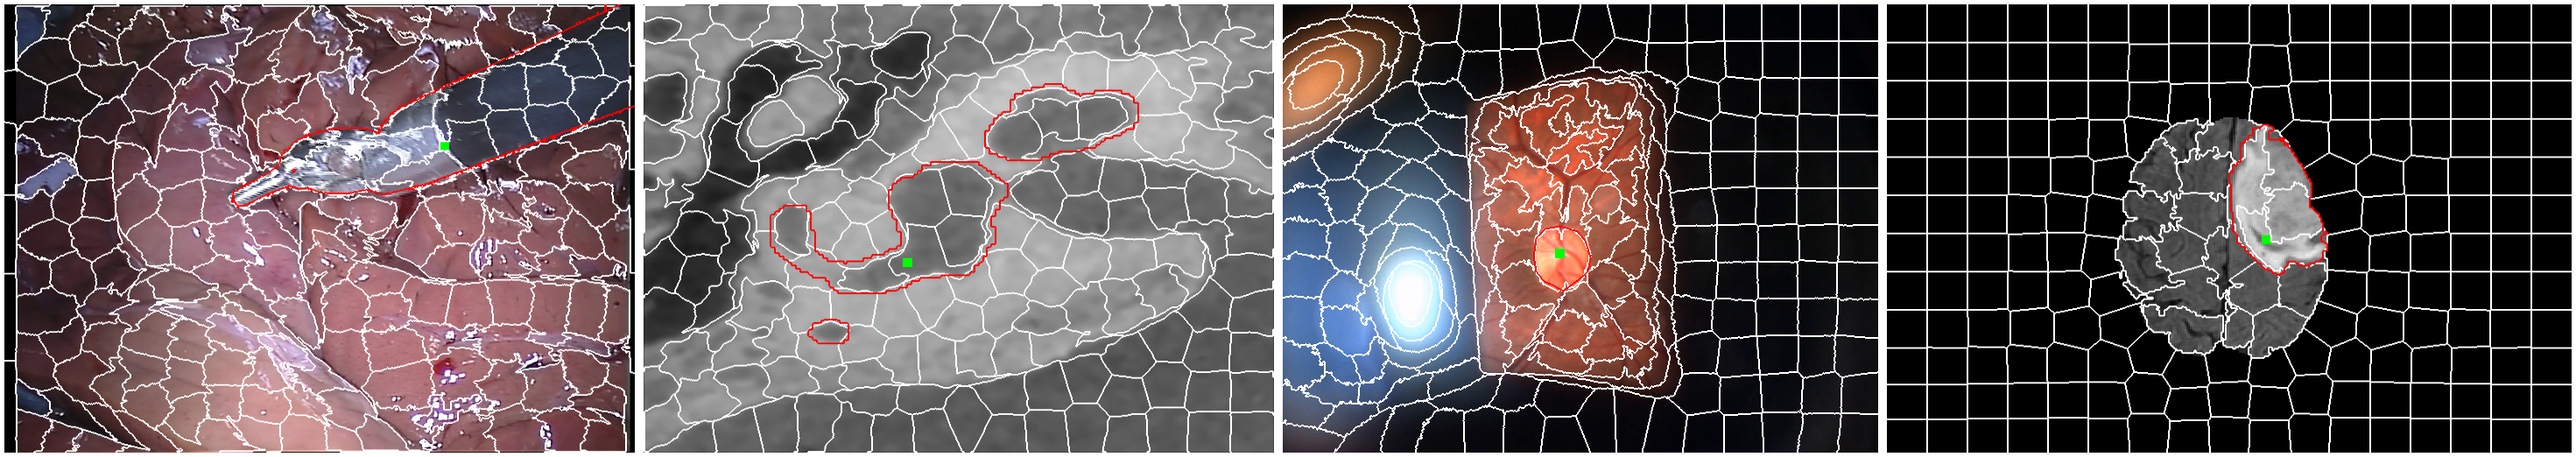
\includegraphics[width=11cm]{prev_sps}
  \caption[Superpixel segmentation example]{Example of superpixel segmentation on each type of sequence. Generated with \cite{achanta12}, with $200$ segments.
  Superpixel contours are in white, ground truth annotation is in red, and user-provided 2D location is in green}
  \label{fig:sp_example}
\end{figure}

Table \ref{tab:sp_errors} shows for each sequence type the maximum F1 score one would obtain while working with SLIC superpixels in a segmentation setup.

Intuitively, this measure increases as the number of superpixels increase.
We use here $N=1200$ superpixels, and note that increasing this value further does not improve the F1-score.

\begin{table}
\centering
\caption{For each type of sequence, we report the maximum F1-score achievable given the early stage superpixel segmentation.}
\label{tab:sp_errors}
\begin{tabular}{lp{1.8cm}}
\toprule
{} &               F1 \\
\midrule
Brain    &  $0.92 \pm 0.02$ \\
Cochlea  &  $0.92 \pm 0.01$ \\
Slitlamp &  $0.92 \pm 0.02$ \\
Tweezer  &  $0.95 \pm 0.01$ \\
\bottomrule
\end{tabular}
\end{table}


\subsection{Activation Maps} \label{ch:act_maps}
To visualize the effect of filters (kernels) in a CNN, one often visualizes their activation during a forward pass.
The examples that follow correspond to the layer where our features are extracted, i.e. the last ReLU of the deepest layer (chapter \ref{feat_extract}). We randomly picked an image, performed a forward pass on a trained \textit{U-Net Rec} model, and visualized $11$ out of the $512$ activation maps. Fig. \ref{fig:activatiom_maps} shows two examples on dataset \textit{MRI Brain A} (Fig. \ref{fig:subfig:activatiom_map_ds09}) and \textit{Slit-Lamp Retina B} (Fig. \ref{fig:subfig:activatiom_map_ds13}). The upper left image shows the input image, and the other plots the activation maps, respectively.

We observe for both examples activation maps that have excitations at the object of interest's location. Thus, the filters are able to capture the foreground region. The fact that no activation maps are fully black indicate that their associated filters effectively contribute to the feature vector. Due to zero-padding used in the convolutional layers, border-effect occur. We will discuss this effect later in chapter \ref{ch:zero_vs_sym_pad}.
\vspace{30pt}

\begin{figure}[!htbp]
  \centering
  \subfloat[Example on \textit{MRI Brain A}]
  {
    \label{fig:subfig:activatiom_map_ds09}
    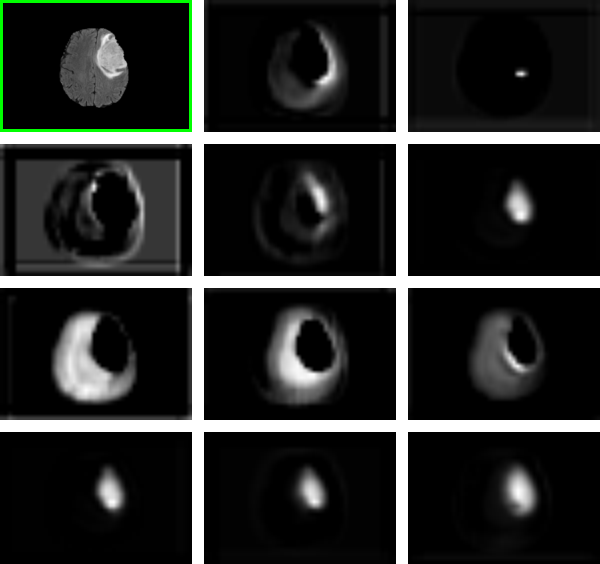
\includegraphics[height=6.2cm]{activation_maps/activations_ds09_0097}
  }
  \hfill
  \subfloat[Example on \textit{Slit-Lamp Retina B}]
  {
    \label{fig:subfig:activatiom_map_ds13}
    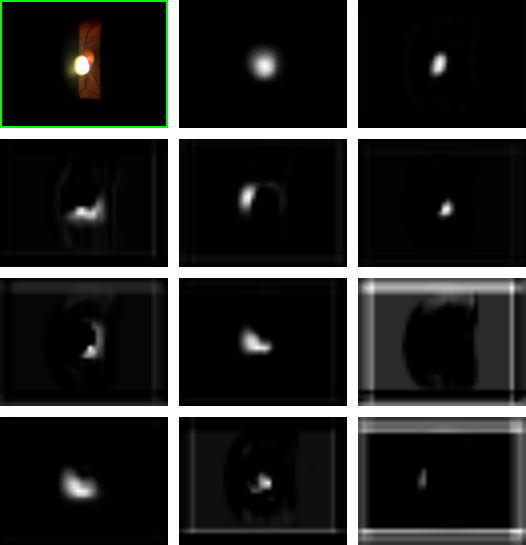
\includegraphics[height=6.2cm]{activation_maps/activations_ds13_0109}
  }
  \caption[Activation maps]{Activation maps of the \textit{U-Net Rec} model for \textit{Brain A} and \textit{Slitlamp B}.
    The upper left image shows the input image.
    The other plots show randomly chosen activation maps, extracted at the bottleneck.}
  \label{fig:activatiom_maps}
\end{figure}

\clearpage
\subsection{Feature Extraction Methods}
We provide results of the evaluation of our feature extraction methods.
The evaluation procedure's configurations are first described.
Second, the numerical values of the parameters of our methods are given.
Third, we show the influence of using data augmentation.
Fourth, we give experimental results on the feature performance vs. training-time.
Fifth, the influence of the selected features of Random Forest is observed.
Sixth, we present an overall ranking of the feature extraction methods in terms of \textit{max F1-Score}.
Last, we investigate the influence of zero-padding.


\subsection{Importance of Data Augmentation} \label{ch:nec_data_gen}
To explore the importance of data augmentation, we trained a \textit{U-Net Rec} model once with standard configuration (use of data generator) and once without using the data generator.
As for all experiments, we performed the training and evaluation with ten repetitions, then took the mean \textit{max F1-Score}.
We performed this experiment on one dataset per image modality. The results are summarized in Tab. \ref{tab:data_gen_nec}.
\vspace{30pt}

\begin{table}[!htbp]
   \centering
   \caption[Importance of data generator]{Influence of data augmentation in terms of mean \textit{max F1-Score} over ten repetitions. A \textit{U-Net Rec} model is trained in standard configuration, i.e. using data agumentation and without using data augmentation.}
   \begin{tabular}{l|*{4}{c|}}
      \toprule
       & \rotatebox[origin=cB]{90}{\parbox[t]{3.2cm}{\hspace{3pt} \textbf{Surgical Video} \hspace*{\fill}}} 
       & \rotatebox[origin=cB]{90}{\parbox[t]{3.2cm}{\hspace{3pt} \textbf{MRI Brain A} \hspace*{\fill}}} 
       & \rotatebox[origin=cB]{90}{\parbox[t]{3.2cm}{\hspace{3pt} \textbf{CT Inner Ear A} \hspace*{\fill}}} 
       & \rotatebox[origin=cB]{90}{\parbox[t]{3.2cm}{\hspace{3pt} \textbf{Slit-Lamp A} \hspace*{\fill}}} \\
      \midrule
      Data Augmentation \textbf{not in use} & 0.9826 & 0.9792 & 0.9587 & 0.9800 \\\midrule
      Data Augmentation \textbf{in use} & 0.9832 & 0.9810 & 0.9621 & 0.9863 \\\midrule\midrule
      \textbf{Gain} by using Data Augmentation & \textbf{0.061\%} & \textbf{0.184\%} & \textbf{0.355\%} & \textbf{0.643\%} \\
      \bottomrule
   \end{tabular}
   \label{tab:data_gen_nec}
\end{table}

\clearpage
\subsection{Performance w.r.t Training Time} \label{sec:perf_vs_training}
We now evaluate the performance of our features with respect to training time.
We trained a \textit{U-Net AE} model for $100$ epochs and run our evaluation pipeline every $10$ epochs.
Similar to all of our evaluations, we did the training and evaluation with ten repetitions to reduce variance.
Fig. \ref{fig:perf_vs_training} shows the mean \textit{max F1-Score} for one dataset per image modality.
We notice that past $20$ epochs the performance stagnates or even decreases for \textit{Cochlea A} dataset.
The next section provides more insight on that particular behaviour.
\vspace{30pt}

\begin{figure}[!htbp]
  \centering
  {
    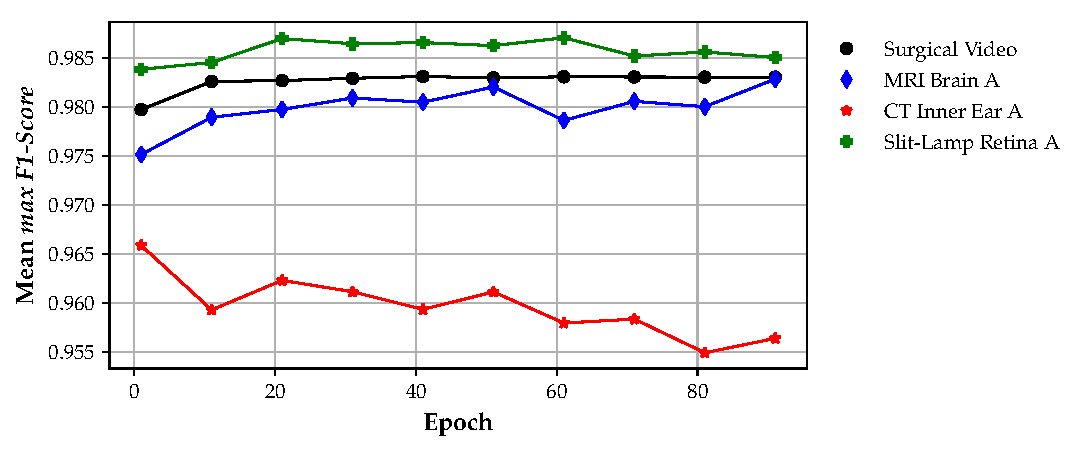
\includegraphics[width=\textwidth]{f1_score_vs_training_time/f1_vs_training_rec}
  }
  \caption[Feature quality vs training time of U-Net Rec model]{Mean \textit{max F1-Score} over ten repetitions w.r.t training time using features from \textit{U-Net AE} for one dataset per image modality.}
  \label{fig:perf_vs_training}
\end{figure}

\clearpage
\subsection{Influence on Random Forest Feature Selection} \label{sec:infl_feat_selection}
Fig. \ref{fig:perf_vs_training_maxfeat} shows a comparison of performances for dataset \textit{Cochlea A} w.r.t parameter $m$, the number of sampled features of the Random Forest (see Sec. \ref{random_forest}).
We observe that setting $m=\sqrt{p}$, as advised by \cite[Ch. 15]{hastie09}, gives higher \textit{max F1-Scores} compared to $m=p$.
Both curves show a decreasing tendency.
\vspace{10pt}

\begin{figure}[!htbp]
  \centering
  {
    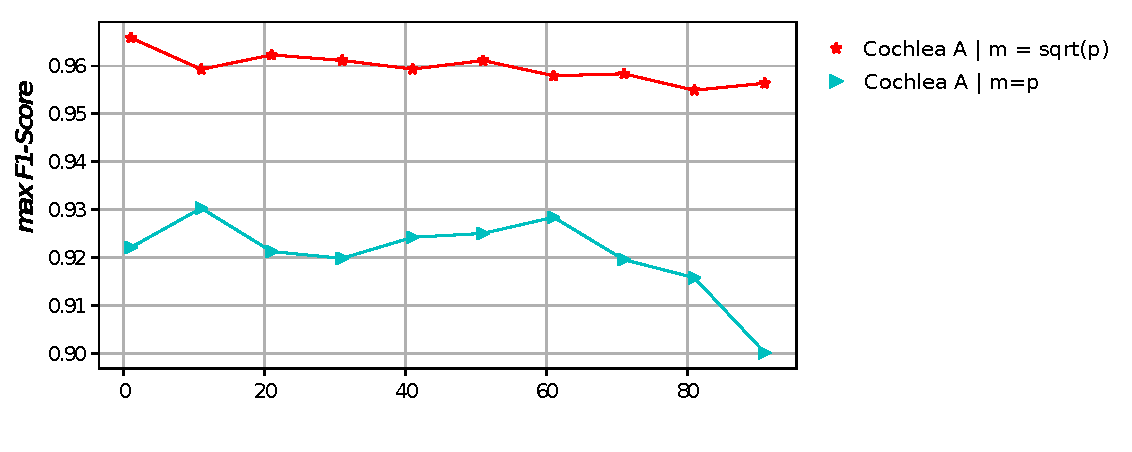
\includegraphics[width=\textwidth]{f1_score_vs_training_time/f1_vs_training_rec_maxfeat}
  }
  \caption[Feature quality vs training time of U-Net Rec model]{Mean \textit{max F1-Score} over ten repetitions w.r.t training time. The graph shows the results of \textit{U-Net Rec} model for dataset \textit{CT Inner Ear A}. The red curve illustrates the result when Random Forest selects $m=\sqrt{p}$ features and the cyan curve when selecting $m=p$.}
  \label{fig:perf_vs_training_maxfeat}
\end{figure}

Based on this observations, we choose to train our U-Net based models for $20$ epochs and set $m=\sqrt{p}$ in the following experiments.
\vspace{20pt}

\subsection{Method Comparison}
Tab. \ref{tab:final_results} summarizes the feature performance for each dataset and method in terms of \textit{max F1-Scores} averaged over ten repetitions.
All best scores per dataset are in red.
For each dataset and method, we performed a two-sided Welch's t-test \cite{welch47} to determine whether the score reached by the individual method is significantly different to the score reached by the best method for that dataset.
All values marked in bold font are not significantly different to the best score for a significance level of $0.05$.
The last row shows how many times the given method did not significantly perform worse than the best method.
We name this score \textit{Top-Sig-Score}.

\begin{table}[!htbp]
   \centering
   \caption[Feature quality]{Performance in terms of \textit{max F1-Scores} averaged over ten repetitions for each dataset and method, respectively. The according standard deviation is given underneath each score. Best scores per dataset are marked in red font. All bold marked scores are not significantly different from the best score when testing by a two-sided Welch's t-test with a significance level of 0.05. The last row shows on how many datasets the specific method was not significantly different to the best method.}
   \begin{tabular}{l|*{9}{c|}}
      \toprule
       & \rotatebox[origin=cB]{90}{\parbox[t]{4cm}{BoVW \hspace*{\fill}}} 
       & \rotatebox[origin=cB]{90}{\parbox[t]{4cm}{ScSP \hspace*{\fill}}} 
       & \rotatebox[origin=cB]{90}{\parbox[t]{4cm}{VGG \hspace*{\fill}}} 
       & \rotatebox[origin=cB]{90}{\parbox[t]{4cm}{U-Net AE \hspace*{\fill}}}
       & \rotatebox[origin=cB]{90}{\parbox[t]{4cm}{U-Net Prior AE \hspace*{\fill}}}
       & \rotatebox[origin=cB]{90}{\parbox[t]{4cm}{U-Net Pred Loc \hspace*{\fill}}}
       & \rotatebox[origin=cB]{90}{\parbox[t]{4cm}{U-Net Pred Loc Frozen \hspace*{\fill}}}
       & \rotatebox[origin=cB]{90}{\parbox[t]{4cm}{U-Net Motion Pred \hspace*{\fill}}}
       & \rotatebox[origin=cB]{90}{\parbox[t]{4cm}{U-Net Motion Pred LSTM \hspace*{\fill}}}  \\
       & \raisebox{-\totalheight}{
\includegraphics[width=0.8cm]{icons/bovw}} 
       & \raisebox{-\totalheight}{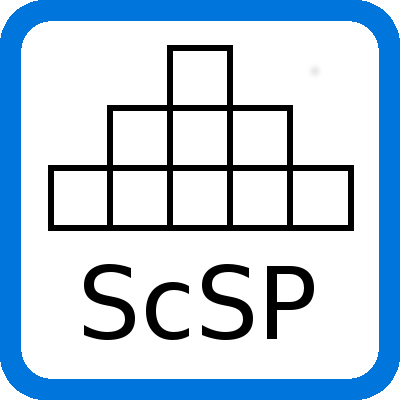
\includegraphics[width=0.8cm]{icons/scsp}} 
       & \raisebox{-\totalheight}{
\includegraphics[width=0.8cm]{icons/vgg}} 
       & \raisebox{-\totalheight}{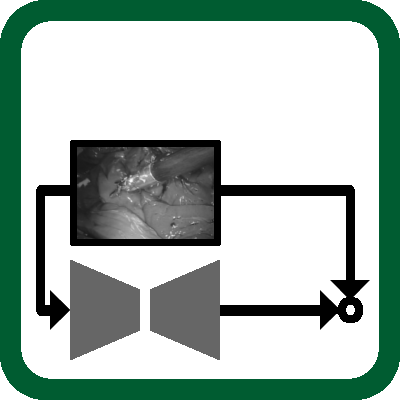
\includegraphics[width=0.8cm]{icons/unet_rec}} 
       & \raisebox{-\totalheight}{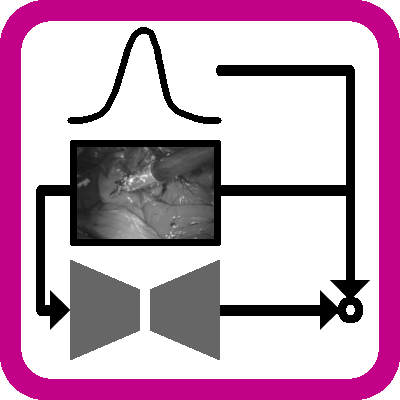
\includegraphics[width=0.8cm]{icons/unet_gaze_rec}} 
       & \raisebox{-\totalheight}{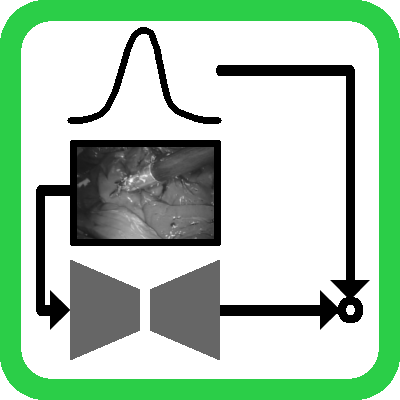
\includegraphics[width=0.8cm]{icons/unet_gaze_prob}} 
       & \raisebox{-\totalheight}{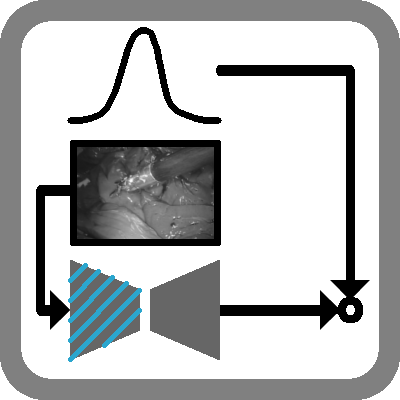
\includegraphics[width=0.8cm]{icons/unet_gaze_prob_freeze}} 
       & \raisebox{-\totalheight}{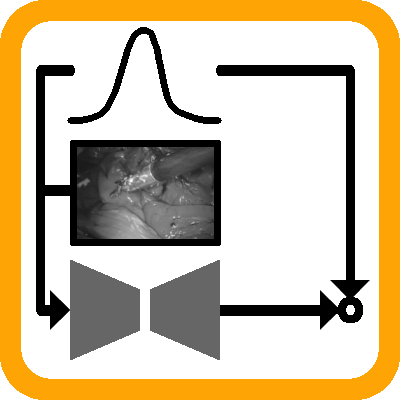
\includegraphics[width=0.8cm]{icons/unet_gaze_prob_concat}} 
       & \raisebox{-\totalheight}{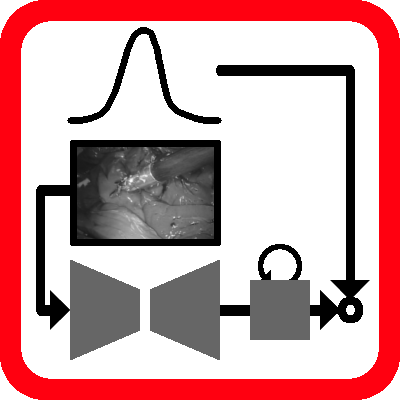
\includegraphics[width=0.8cm]{icons/unet_gaze_prob_lstm}}\\
      \midrule\midrule
      {\scriptsize Surgical Video} & \scriptsize 0.6649 & \scriptsize 0.8998 & \scriptsize 0.9647 & \textbf{\scriptsize 0.9830} & {\color{red} \textbf{\scriptsize 0.9832}} & \scriptsize 0.9791 & \scriptsize 0.9811 & \scriptsize 0.9776 & \scriptsize 0.9807 \\[-4pt]
       & \tiny $\pm$6.24e-4 & \tiny $\pm$6.04e-4 & \tiny $\pm$3.87e-4 & \tiny $\pm$4.84e-4 & \tiny $\pm$4.22e-4 & \tiny $\pm$1.84e-3 & \tiny $\pm$4.78e-4 & \tiny $\pm$2.93e-3 & \tiny $\pm$7.21e-4 \\\midrule\midrule
      {\scriptsize MRI Brain A} & \scriptsize 0.3163 & \scriptsize 0.9288 & \scriptsize 0.9666 & \textbf{\scriptsize 0.9774} & {\color{red} \textbf{\scriptsize 0.9810}} & \scriptsize 0.9764 & \textbf{\scriptsize 0.9806} & \scriptsize 0.9673 & \textbf{\scriptsize 0.9794} \\[-4pt]
       & \tiny $\pm$3.61e-3 & \tiny $\pm$5.05e-3 & \tiny $\pm$2.10e-3 & \tiny $\pm$4.65e-3 & \tiny $\pm$3.95e-3 & \tiny $\pm$3.30e-3 & \tiny $\pm$3.28e-3 & \tiny $\pm$8.90e-3 & \tiny $\pm$5.02e-3 \\\midrule
      {\scriptsize MRI Brain B} & \scriptsize 0.7502 & \scriptsize 0.8568 & \scriptsize 0.8911 & \textbf{\scriptsize 0.9232} & \textbf{\scriptsize 0.9292} & \scriptsize 0.9142 & \textbf{\scriptsize 0.9253} & {\color{red} \textbf{\scriptsize 0.9297}} & \scriptsize 0.9201 \\[-4pt]
       & \tiny $\pm$8.20e-3 & \tiny $\pm$7.36e-3 & \tiny $\pm$3.88e-3 & \tiny $\pm$5.63e-3 & \tiny $\pm$3.74e-3 & \tiny $\pm$8.59e-3 & \tiny $\pm$4.83e-3 & \tiny $\pm$7.09e-3 & \tiny $\pm$7.90e-3 \\\midrule
      {\scriptsize MRI Brain C} & \scriptsize 0.7911 & \scriptsize 0.8957 & \scriptsize 0.9345 & \textbf{\scriptsize 0.9766} & \textbf{\scriptsize 0.9742} & \scriptsize 0.9695 & {\color{red} \textbf{\scriptsize 0.9774}} & \textbf{\scriptsize 0.9742} & \scriptsize 0.9729 \\[-4pt]
       & \tiny $\pm$7.21e-3 & \tiny $\pm$2.66e-3 & \tiny $\pm$3.28e-3 & \tiny $\pm$3.75e-3 & \tiny $\pm$3.31e-3 & \tiny $\pm$2.96e-3 & \tiny $\pm$2.11e-3 & \tiny $\pm$5.15e-3 & \tiny $\pm$4.03e-3 \\\midrule
      {\scriptsize MRI Brain D} & \scriptsize 0.7035 & \scriptsize 0.7764 & \scriptsize 0.8548 & {\color{red} \textbf{\scriptsize 0.9470}} & \textbf{\scriptsize 0.9463} & \scriptsize 0.9207 & \scriptsize 0.9247 & \scriptsize 0.9293 & \scriptsize 0.9276 \\[-4pt]
       & \tiny $\pm$1.27e-2 & \tiny $\pm$6.67e-3 & \tiny $\pm$6.11e-3 & \tiny $\pm$5.42e-3 & \tiny $\pm$4.67e-3 & \tiny $\pm$5.48e-3 & \tiny $\pm$5.48e-3 & \tiny $\pm$4.51e-3 & \tiny $\pm$5.00e-3 \\\midrule
      {\scriptsize MRI Brain (B-D)} & \scriptsize 0.6753 & \scriptsize 0.8046 & \scriptsize 0.8640 & {\color{red} \textbf{\scriptsize 0.9482}} & \textbf{\scriptsize 0.9463} & \scriptsize 0.9167 & \scriptsize 0.9399 & \scriptsize 0.9236 & \scriptsize 0.9310 \\[-4pt]
       & \tiny $\pm$4.83e-3 & \tiny $\pm$1.67e-3 & \tiny $\pm$2.61e-3 & \tiny $\pm$4.65e-3 & \tiny $\pm$3.80e-3 & \tiny $\pm$1.30e-2 & \tiny $\pm$3.40e-3 & \tiny $\pm$5.42e-3 & \tiny $\pm$1.16e-2 \\\midrule\midrule
      {\scriptsize CT Inner Ear A} & \scriptsize 0.5527 & \scriptsize 0.8680 & \scriptsize 0.7400 & \textbf{\scriptsize 0.9624} & \textbf{\scriptsize 0.9621} & \scriptsize 0.9565 & \scriptsize 0.9554 & \textbf{\scriptsize 0.9660} & {\color{red} \textbf{\scriptsize 0.9686}} \\[-4pt]
       & \tiny $\pm$1.24e-2 & \tiny $\pm$1.02e-2 & \tiny $\pm$6.09e-3 & \tiny $\pm$4.75e-3 & \tiny $\pm$6.38e-3 & \tiny $\pm$8.60e-3 & \tiny $\pm$6.42e-3 & \tiny $\pm$7.20e-3 & \tiny $\pm$8.12e-3 \\\midrule
      {\scriptsize CT Inner Ear B} & \scriptsize 0.4659 & \scriptsize 0.8372 & \scriptsize 0.7786 & {\color{red} \textbf{\scriptsize 0.9628}} & \textbf{\scriptsize 0.9623} & \scriptsize 0.9481 & \scriptsize 0.9443 & \scriptsize 0.9560 & \scriptsize 0.9476 \\[-4pt]
       & \tiny $\pm$1.78e-2 & \tiny $\pm$5.55e-3 & \tiny $\pm$5.11e-3 & \tiny $\pm$3.34e-3 & \tiny $\pm$1.41e-3 & \tiny $\pm$7.64e-3 & \tiny $\pm$6.63e-3 & \tiny $\pm$4.61e-3 & \tiny $\pm$1.35e-2 \\\midrule\midrule
      {\scriptsize Slit-Lamp A} & \scriptsize 0.8912 & \scriptsize 0.9742 & \scriptsize 0.9784 & \textbf{\scriptsize 0.9845} & \textbf{\scriptsize 0.9863} & \scriptsize 0.9839 & {\color{red} \textbf{\scriptsize 0.9890}} & \scriptsize 0.9788 & \scriptsize 0.9780 \\[-4pt]
       & \tiny $\pm$9.97e-3 & \tiny $\pm$5.34e-3 & \tiny $\pm$3.57e-3 & \tiny $\pm$5.20e-3 & \tiny $\pm$3.36e-3 & \tiny $\pm$4.06e-3 & \tiny $\pm$2.74e-3 & \tiny $\pm$8.12e-3 & \tiny $\pm$4.20e-3 \\\midrule
      {\scriptsize Slit-Lamp B} & \scriptsize 0.6454 & \textbf{\scriptsize 0.9909} & \scriptsize 0.9775 & \scriptsize 0.9687 & \scriptsize 0.9747 & \textbf{\scriptsize 0.9888} & \scriptsize 0.9707 & {\color{red} \textbf{\scriptsize 0.9913}} & \scriptsize 0.9827 \\[-4pt]
       & \tiny $\pm$1.29e-2 & \tiny $\pm$2.48e-3 & \tiny $\pm$4.05e-3 & \tiny $\pm$8.44e-3 & \tiny $\pm$6.62e-3 & \tiny $\pm$4.32e-3 & \tiny $\pm$5.33e-3 & \tiny $\pm$2.43e-3 & \tiny $\pm$4.05e-3 \\\midrule
      {\scriptsize Slit-Lamp C} & \scriptsize 0.8681 & {\color{red} \textbf{\scriptsize 0.9870}} & \scriptsize 0.9724 & \textbf{\scriptsize 0.9862} & \textbf{\scriptsize 0.9826} & \scriptsize 0.9686 & \textbf{\scriptsize 0.9792} & \scriptsize 0.9736 & \scriptsize 0.9707 \\[-4pt]
       & \tiny $\pm$5.63e-3 & \tiny $\pm$3.43e-3 & \tiny $\pm$4.55e-3 & \tiny $\pm$7.43e-3 & \tiny $\pm$5.50e-3 & \tiny $\pm$1.33e-2 & \tiny $\pm$8.54e-3 & \tiny $\pm$9.44e-3 & \tiny $\pm$7.07e-3 \\\midrule
      {\scriptsize Slit-Lamp D} & \scriptsize 0.7752 & \scriptsize 0.9837 & \scriptsize 0.9460 & \textbf{\scriptsize 0.9874} & \scriptsize 0.9852 & \scriptsize 0.9764 & {\color{red} \textbf{\scriptsize 0.9918}} & \scriptsize 0.9800 & \scriptsize 0.9780 \\[-4pt]
       & \tiny $\pm$8.40e-3 & \tiny $\pm$2.03e-3 & \tiny $\pm$3.89e-3 & \tiny $\pm$6.05e-3 & \tiny $\pm$6.03e-3 & \tiny $\pm$1.16e-2 & \tiny $\pm$4.18e-3 & \tiny $\pm$5.49e-3 & \tiny $\pm$3.84e-3 \\\midrule
      {\scriptsize Slit-Lamp (A-D)} & \scriptsize 0.7663 & \scriptsize 0.9729 & \scriptsize 0.9507 & \textbf{\scriptsize 0.9779} & {\color{red} \textbf{\scriptsize 0.9785}} & \scriptsize 0.9669 & \textbf{\scriptsize 0.9767} & \scriptsize 0.9715 & \scriptsize 0.9641 \\[-4pt]
       & \tiny $\pm$9.04e-3 & \tiny $\pm$1.41e-3 & \tiny $\pm$2.57e-3 & \tiny $\pm$3.32e-3 & \tiny $\pm$3.19e-3 & \tiny $\pm$1.10e-2 & \tiny $\pm$3.22e-3 & \tiny $\pm$6.59e-3 & \tiny $\pm$5.98e-3 \\\bottomrule\toprule
      {\scriptsize \textbf{Top-Sig-Score}} & 0 & 2 & 0 & 12 & 11 & 1 & 7 & 4 & 2 \\\bottomrule
   \end{tabular}
   \label{tab:final_results}
\end{table}

Surprisingly, one baseline method (\textit{ScSP}) reached two times the \textit{Top-Sig-Score}.
Both times in a slit-lamp sequence.
Fig. \ref{fig:curves_ds14} gives detailed results on the \textit{Slit-Lamp Retina C} dataset.
Fig. \ref{subfig:pr_curve_ds14} shows the PR-Curve as an average over all ten repetitions.
Fig. \ref{subfig:reprod_ds14} illustrates the distribution of the \textit{max F1-scores} over ten repetitions as a box-plot.

Similarly to Fig. \ref{fig:curves_ds14}, we show in Fig. \ref{fig:curves_ds16} detailed results of dataset \textit{MRI Brain B} to illustrate the improvement obtained by U-Net based methods on that image modality.

\begin{figure}[!htbp]
  \centering
  \subfloat[\textit{PR-Curves} of dataset \textit{Slitlamp C}]
  {
    \label{subfig:pr_curve_ds14}
    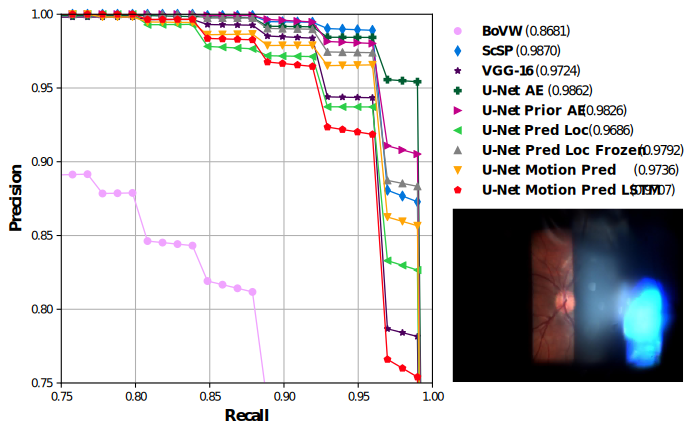
\includegraphics[width=12cm]{final_eval/ds14_pr}
  }
  \\[30pt]
  \subfloat[\textit{Max F1-Scores} of dataset \textit{Slitlamp C}]
  {
    \label{subfig:reprod_ds14}
    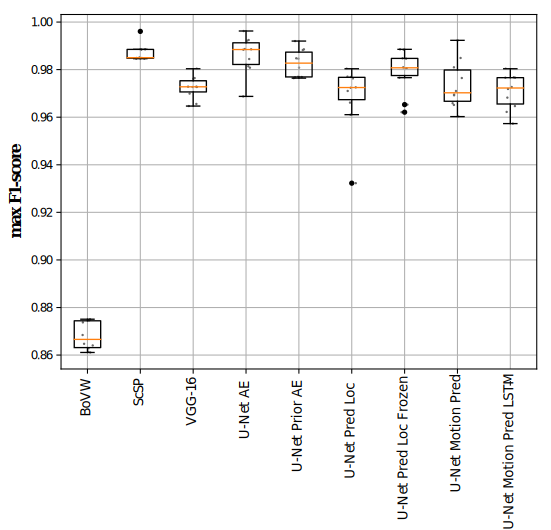
\includegraphics[width=10cm]{final_eval/ds14_reprod}
  }
  \caption[Detailed results of dataset \textit{Slitlamp C}]{Detailed results of dataset \textit{Slitlamp C}. (a) \textit{PR-Curves} averaged on ten repetitions (b) Box-plot of \textit{max F1-Score} on each fold (median and standard deviation)}
  \label{fig:curves_ds14}  
\end{figure}

\clearpage
\begin{figure}[!htbp]
  \centering
  \subfloat[\textit{PR-Curves} of dataset \textit{MRI Brain B} with an example image]
  {
    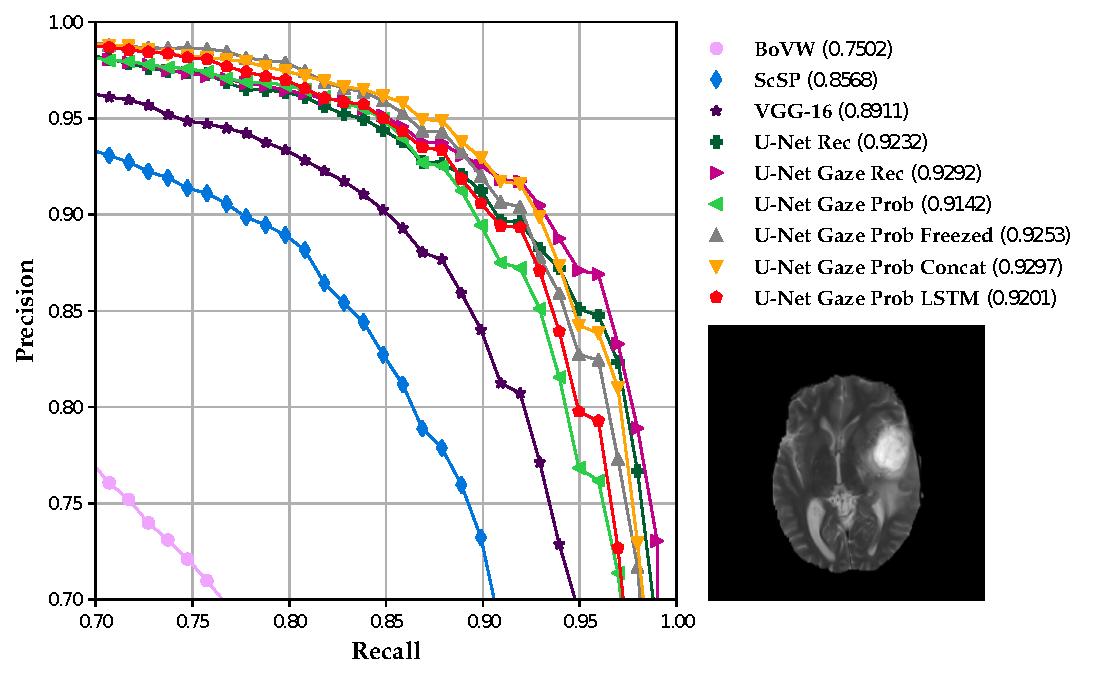
\includegraphics[width=12cm]{final_eval/ds16_pr}
  }
  \\[20pt]
  \subfloat[\textit{Max F1-Scores} of dataset \textit{MRI Brain B}]
  {
    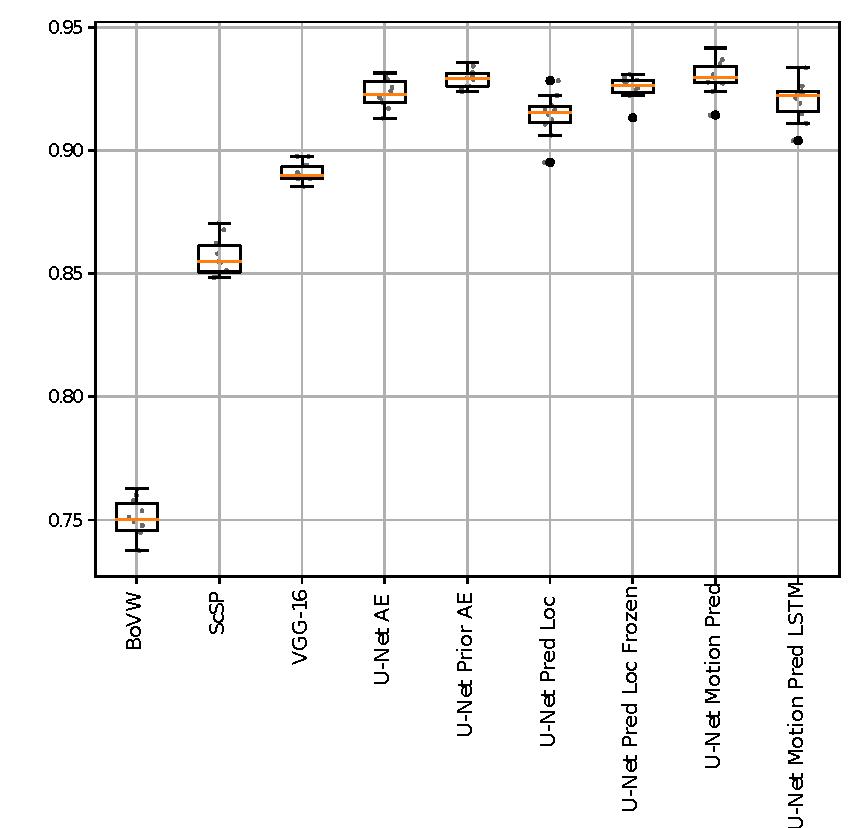
\includegraphics[width=10cm]{final_eval/ds16_reprod}
  }
  \caption[Detailed results of dataset \textit{Slit-Lamp Retina C}]{Detailed results of dataset \textit{MRI Brain B}. (a) \textit{PR-Curves} averaged on ten repetitions. \textit{Max F1-Scores} are given in the legends. (b) Box-plot of \textit{max F1-Score} on each repetition. The median is drawn in orange.}
  \label{fig:curves_ds16}  
\end{figure}

\subsection{Zero-Padding vs. Symmetric-Padding} \label{ch:zero_vs_sym_pad}
To investigate the influence of the border-effect due to zero-padding, we retrained our best model \textit{U-Net Pred Loc} using symmetric-padding for all convolutional layers.
When padding the input with symmetric property, the added pixel rows and columns are a mirror reflection of the input itself.
We trained the model on one dataset per image modality.
Fig. \ref{fig:activatiom_maps_sym} shows the activation maps in both setups on \textit{Brain A}.
The activation maps at the output of the bottleneck (see chapter \ref{ch:act_maps}).

\begin{figure}[!htbp]
  \centering
  \subfloat[Activation maps with zero-padding]
  {
    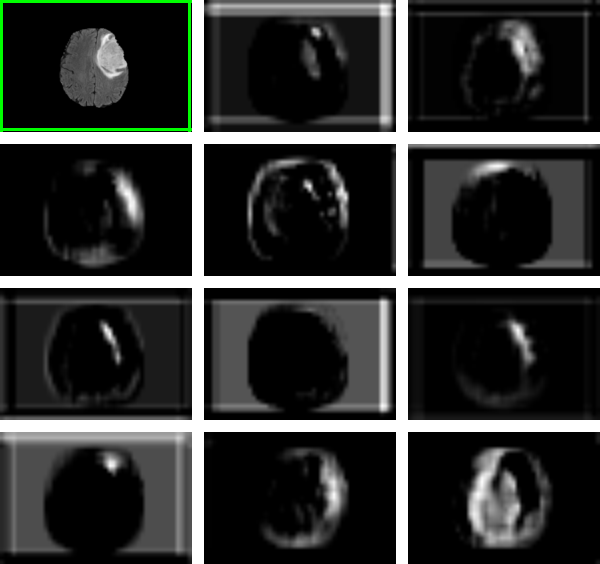
\includegraphics[height=5.8cm]{activation_maps/activations_ds09_0097_gaze_rec}
  }
  \hfill
  \subfloat[Activation maps with symmetric-padding]
  {
    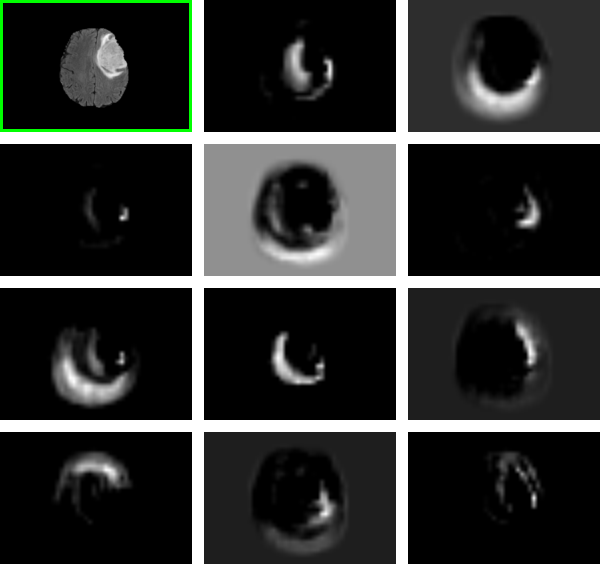
\includegraphics[height=5.8cm]{activation_maps/activations_ds09_0097_gaze_rec_sympadded}
  }
  \caption[Activation maps symmetric padding]{Activation maps of a trained \textit{U-Net Gaze Rec} model with (a) zero-padding (standard configuration) and (b) symmetric-padding for the convolutional layers. The upper left image shows the passed image from \textit{MRI Brain A} datasets. The other $11$ plots show some randomly chosen activation maps, extracted at the deepest level after the last ReLU.}
  \label{fig:activatiom_maps_sym}
\end{figure}

Tab. \ref{tab:zero_vs_sym_padd} shows the mean \textit{max F1-Scores} over ten repetitions using zero-padding and symmetric-padding. We note no substantial improvement.

\begin{table}[!htbp]
   \centering
   \caption[Zero-padding vs. symmetric-padding]{Comparison of zero-padding vs. symmetric-padding using \textit{U-Net Prior AE} model.
     We give the mean \textit{max F1-Scores} for one dataset per image modality over ten repetitions.
     The last column indicates the improvement due to symmetric-padding.}
   \small
   \begin{tabular}{l|c|c||c|}
      \toprule
       & \Gape[6pt][6pt]{\rotatebox[origin=cB]{90}{\parbox[t]{2.6cm}{U-Net Prior AE \\ \textit{\textbf{Zero-Pad}\hspace*{\fill}}}}}
       & \rotatebox[origin=cB]{90}{\parbox[t]{2.6cm}{U-Net Prior AE \\ \textit{\textbf{Symmetric-Pad}\hspace*{\fill}}}}
       & \rotatebox[origin=cB]{90}{\parbox[t]{2.6cm}{\textbf{Improvement\hspace*{\fill}}}} \\
      \midrule
      \textbf{Tweezer} & 0.9832 & 0.9823  & \textbf{-0.091\%} \\\midrule
      \textbf{Brain A} & 0.9810 & 0.9830 &  \textbf{+0.203\%} \\\midrule
%      {\scriptsize MRI Brain B} & \scriptsize 0.9292 & \scriptsize 0.9278 & \scriptsize -0.0014 \\\midrule
%      {\scriptsize MRI Brain C} & \scriptsize 0.9742 & \scriptsize 0.9760 & \scriptsize +0.0018 \\\midrule
%      {\scriptsize MRI Brain D} & \scriptsize 0.9463 & \scriptsize 0.9470 & \scriptsize +0.0006 \\\midrule
%      {\scriptsize MRI Brain (B-D)} & \scriptsize 0.9463 & \scriptsize 0.9431 & \scriptsize -0.0032 \\\midrule\midrule
      \textbf{Cochlea A} & 0.9621 & 0.9535 & \textbf{-0.893\%} \\\midrule
%      {\scriptsize CT Inner Ear B} & \scriptsize 0.9623 & \scriptsize 0.9566 & \scriptsize -0.0057 \\\midrule\midrule
      \textbf{Slitlamp A} & 0.9863 & 0.9860 & \textbf{-0.03\%} \\
%      {\scriptsize Slit-Lamp B} & \scriptsize 0.9747 & \scriptsize 0.9796 & \scriptsize +0.0049 \\\midrule
%      {\scriptsize Slit-Lamp C} & \scriptsize 0.9826 & \scriptsize 0.9846 & \scriptsize +0.002 \\\midrule
%      {\scriptsize Slit-Lamp D} & \scriptsize 0.9852 & \scriptsize 0.9886 & \scriptsize +0.0034 \\\midrule
%      {\scriptsize Slit-Lamp A-D} & \scriptsize 0.9785 & \scriptsize 0.9763 & \scriptsize -0.0022 \\
      \bottomrule
   \end{tabular}
   \label{tab:zero_vs_sym_padd}
\end{table}

%%% Local Variables:
%%% mode: latex
%%% TeX-master: "../../main"
%%% End:
